% !TEX program = xelatex

\documentclass[10pt,aspectratio=169,mathserif]{beamer}
%设置为 Beamer 文档类型,设置字体为 10pt,长宽比为16:9,数学字体为 serif 风格

%%%%-----导入宏包-----%%%%
\usepackage{ecnu}			%导入 CCNU 模板宏包
\usepackage{ctex}			 %导入 ctex 宏包,添加中文支持
\usepackage{amsmath,amsfonts,amssymb,bm}   %导入数学公式所需宏包
\usepackage{color}			 %字体颜色支持
\usepackage{graphicx,hyperref,url}
\usepackage{caption}
\usepackage[most]{tcolorbox}
\usepackage{colortbl}
\usepackage{indentfirst}
\usepackage{setspace}
\usepackage{booktabs}
\usepackage{geometry}
\tcbuselibrary{skins, breakable, theorems, fitting}

\usepackage{tikz}
\usetikzlibrary{positioning}
\tikzset{>=stealth}

%%%%%%%%%%%%%%%%%%

%%%%%%%%%%%%%%%%%%

\beamertemplateballitem		%设置 Beamer 主题

\setbeamertemplate{navigation symbols}{}		% 取消右下角导航栏

%%%%------------------------%%%%%
\catcode`\。=\active         %或者=13
\newcommand{。}{.}
%将正文中的“。”号转换为“.”。
%%%%%%%%%%%%%%%%%%%%%

%%%%----首页信息设置----%%%%
\title[Design and Implementation of Othello Based on Reinforcement Learning]{基于强化学习的黑白棋的设计与实现}
\subtitle{Design and Implementation of Othello Based on Reinforcement Learning}
%%%%----标题设置


\author[by im0qianqian]{
  Zhao Qian \\\medskip
  {\small {Adviser: Jerry Wang}} \\
}
%%%%----个人信息设置

\institute[YTU]{
  Yantai University \\
  School of Computer and Control Engineering}
%%%%----机构信息

\date[2019.05.30]{
  2019.05.30}
%%%%----日期信息

\begin{document}

\begin{frame}
  \titlepage
\end{frame}				%生成标题页

% \section{大纲}
% \begin{frame}
%   \frametitle{Outline}
%   \tableofcontents[]
% \end{frame}				%生成提纲页


\section{研究动机}
\begin{frame}
  \frametitle{Why Reversi and Prior Work}
  \begin{columns}
    \column{.55\textwidth}
    \begin{tcolorbox}[standard jigsaw,title=Why Reversi?,height=6.5cm,opacityback=.5,colbacktitle=black!70!white,colframe=white]
      % \begin{block}{Why Reversi?}
      \begin{figure}[tb]
        \centering
        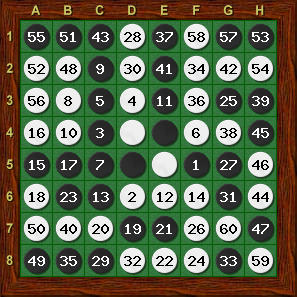
\includegraphics[width=.5\textwidth]{img/othello.jpg}
      \end{figure}
      \begin{footnotesize}
        \begin{itemize}
          \item {\songti 以往算法的设计中大都使用博弈树搜索的方法}
          \item {\songti 2017 年 AlphaGo Zero 出现了}
          \item {\songti 打算将这种思路扩展到黑白棋中}
        \end{itemize}
      \end{footnotesize}
      % \end{block}
    \end{tcolorbox}
    \column{.55\textwidth}
    \begin{tcolorbox}[standard jigsaw,title=Prior Work,height=6.5cm,opacityback=.5,colbacktitle=black!70!white,colframe=white]
      % \begin{block}{Prior Work}
      \begin{footnotesize}
        \textbf{Minimax Tree Search + Alpha-Beta pruning}
        \begin{itemize}
          \item {\songti 搜索空间巨大(随搜索层数指数级增加)}
          \item {\songti 棋力受限于搜索的层数(理想时间内很难提高)}
          \item {\songti 棋力受限于设计者的能力(如估值函数的设计)}
        \end{itemize}
        \vspace{1cm}
        \textbf{Monte Carlo Tree Search}
        \begin{itemize}
          \item {\songti 无需任何领域知识便可工作}  % MCTS 不要求任何关于给定的领域策略或者具体实践知识来做出合理的决策。这个算法可以在没有任何关于博弈游戏除基本规则外的知识的情况下进行有效工作;这意味着一个简单的 MCTS 实现可以重用在很多的博弈游戏中,只需要进行微小的调整,所以这也使得 MCTS 是对于一般的博弈游戏的很好的方法。
          \item {\songti 非对称式增长,算法会频繁地访问“更感兴趣”的节点,并聚焦搜索空间于更加相关树的部分}
          \item {\songti 算法可在任何时间终止,并返回当前最优的估计}
        \end{itemize}
      \end{footnotesize}
      % \end{block}
    \end{tcolorbox}
  \end{columns}
\end{frame}

\section{游戏规则}
\begin{frame}
  \frametitle{Reversi: Basic Rules}
  \begin{columns}
    \column{.55\textwidth}
    \begin{tcolorbox}[standard jigsaw,title=How to play,height=6.5cm,opacityback=.5,colbacktitle=black!70!white,colframe=white]
      \begin{minipage}[b]{0.30\textwidth}
        \flushleft
        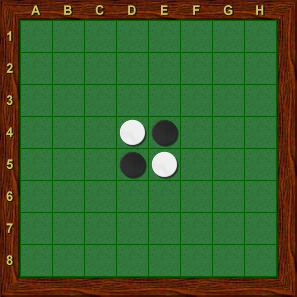
\includegraphics[height=1.0\textwidth]{img/othello_init.jpg}
      \end{minipage}
      \begin{minipage}[b]{.65\textwidth}
        \flushright
        \begin{footnotesize}
          \begin{itemize}
            \item {\songti 棋盘 $8 \times 8$ 大小}
            \item {\songti E4、D5 为黑棋}
            \item {\songti D4、E5 为白棋}
            \item {\songti 执黑先手}
          \end{itemize}
          \medskip
        \end{footnotesize}
      \end{minipage}
      \tcblower
      \begin{minipage}[b]{.55\textwidth}
        \flushleft
        \begin{footnotesize}
          \begin{itemize}
            \item {\songti 落子必须在一空位}
            \item {\songti 落子必须造成翻转}
            \item {\songti 无子可走则本轮 pass}
            \item {\songti 有子可走则必须走棋}
          \end{itemize}
        \end{footnotesize}
        \medskip
      \end{minipage}
      \begin{minipage}[b]{0.4\textwidth}
        \flushright
        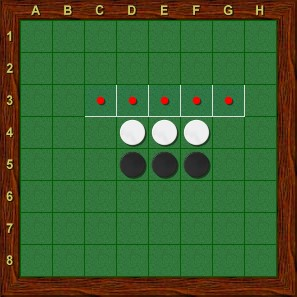
\includegraphics[height=1.0\textwidth]{img/othello1.jpg}
      \end{minipage}
    \end{tcolorbox}
    \column{.55\textwidth}
    \begin{tcolorbox}[standard jigsaw,title=How to win,height=6.5cm,opacityback=.5,colbacktitle=black!70!white,colframe=white]
      \begin{figure}[tb]
        \centering
        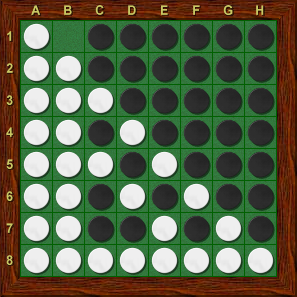
\includegraphics[width=.5\textwidth]{img/othello_end.jpg}
      \end{figure}
      \begin{footnotesize}
        \small \textbf{获胜条件:}
        \begin{enumerate}
          \item \songti 双方都无子可下
          \item \songti 棋子数目多者获胜,若相等为平局
        \end{enumerate}
      \end{footnotesize}
    \end{tcolorbox}
  \end{columns}
\end{frame}

\section{强化学习}
\begin{frame}
  \frametitle{Reinforcement Learning}
  \setlength{\parindent}{2em}\textrm{\songti 强化学习解决一类序贯决策问题,它不关心输入的数据长什么样子,它只关心当前采取什么样的行动才能使得最终的回报最大\\}
  \begin{minipage}{.5\textwidth}
    \flushleft
    \begin{figure}
      \flushleft
      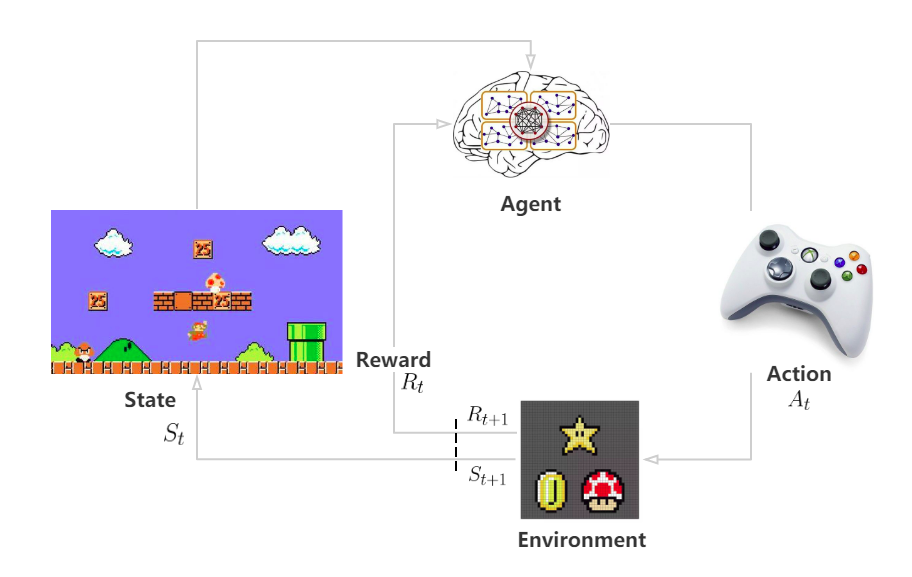
\includegraphics[width=8cm]{img/RL.png}
    \end{figure}
  \end{minipage}
  \begin{minipage}{0.4\textwidth}
    \begin{figure}
      \flushright
      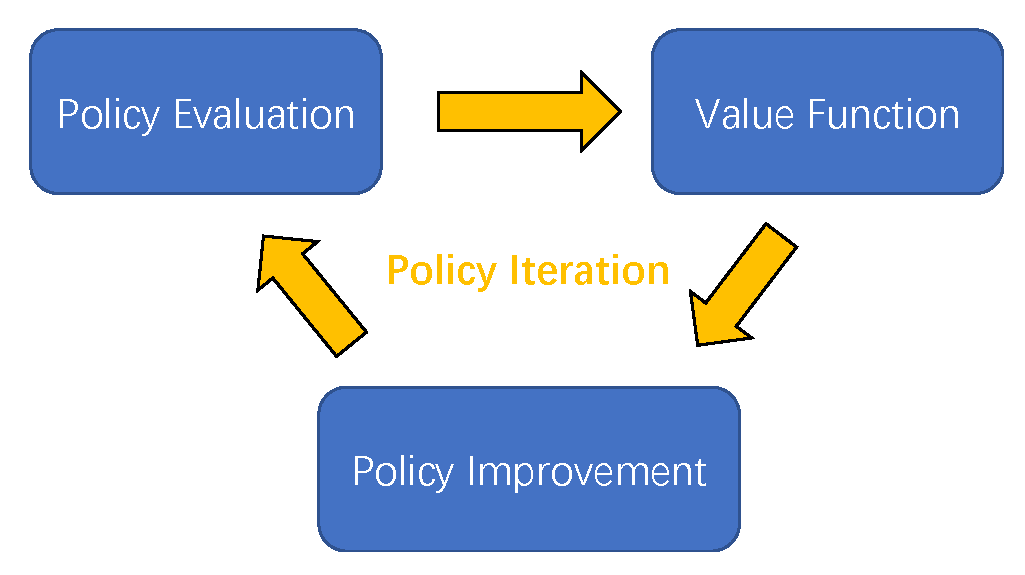
\includegraphics[width=5cm]{img/CoreRLConcepts.pdf}
    \end{figure}
  \end{minipage}
\end{frame}

\section{系统设计}
\subsection{整体架构}

\begin{frame}
  \frametitle{Structure Breakdown}
  \begin{tcolorbox}[standard jigsaw,title=\small 神经网络 $f_\theta$ (predict),titlerule=-1.1em,opacityback=.5,colbacktitle=black!70!white,colframe=white]
      \begin{columns}[t]
        \column{.3\textwidth}
        \flushright
        \text{$(\vec{p},v) = f_\theta(s)$}
        \column{.7\textwidth}
      \centering
    \begin{itemize}
    \item {\footnotesize $\vec{p}_\theta(s_t):$ 当前玩家在状态 $s_t$ 下选择每个动作的概率}
    \item {\footnotesize $v_\theta(s_t):$ 当前玩家在状态 $s_t$ 下获胜的概率估计}
    \end{itemize}
    \end{columns}
    \end{tcolorbox}
    \begin{minipage}{.4\textwidth}
      \begin{figure}
        \includegraphics[width=6cm]{img/CoreRLConcepts2.pdf}
      \end{figure}
    \end{minipage}
  \begin{minipage}{0.55\textwidth}
    \begin{figure}
      \begin{tcolorbox}[standard jigsaw,title=\footnotesize Policy Evaluation,titlerule=-.5em,opacityback=.5,colbacktitle=black!70!white,colframe=white,add to width=.5cm]
      \text{\footnotesize $f_\theta(s) \stackrel{(\vec{p}, v)}{\longrightarrow} {\rm MCTS} \stackrel{\vec{\pi}_t}{\longrightarrow} action$}
      \text{\footnotesize \songti 到达终止态 $s_T$ 获得本局胜利者 $Z$}
      \end{tcolorbox}
      \begin{tcolorbox}[standard jigsaw,title=\footnotesize Policy Improvement,titlerule=-.5em,opacityback=.5,colbacktitle=black!70!white,colframe=white] 
        \text{\footnotesize \songti 通过 self play 得到一组 train data}
        \text{\footnotesize \songti 使用 train data 训练神经网络得出新 model}
        \text{\footnotesize \songti 新旧 model 进行对抗判断胜率是否超过阈值需要更新}
      \end{tcolorbox}
    \end{figure}
  \end{minipage}
\end{frame}

\subsection{兼具策略评估与价值评估的神经网络}
\begin{frame}
  \frametitle{Neural Policy and Value Network}
  \begin{tcolorbox}[standard jigsaw,title=\small 神经网络 $f_\theta$ (train),titlerule=0em,opacityback=.5,colbacktitle=black!70!white,colframe=white]
      \begin{columns}
        \column{.5\textwidth}
         {\footnotesize Input: ${\rm train\ data\ }(s_t, \vec{\pi}_t, z_t)$\\}
         {\footnotesize ToDo: 最小化 $\vec{p}_\theta(s_t)$ 与 $\vec{\pi}_t$,$v_\theta(s_t)$ 与 $z_t$ 间的差距}
      \column{.5\textwidth}
        \begin{equation*}
          \footnotesize Loss = \sum_t (v_\theta(s_t) - z_t)^2 - \vec{\pi}_t \cdot \log(\vec{p}_\theta(s_t))
        \end{equation*}
    \end{columns}
    \end{tcolorbox}
\end{frame}

\subsection{使用蒙特卡洛搜索进行策略改进}
\begin{frame}
  \frametitle{Monte Carlo Tree Search for Policy Improvement}
  \textbf{Sample Text\\}
  \noindent\textbf{Sample Text\\}
\end{frame}

\section{实验分析}
\begin{frame}
  \frametitle{Experiments and Analysis}
  \text{\heiti 一块 Tesla T4 中训练了 150h,共迭代 120 次,其中成功 29 次,平均每次成功迭代耗时 5.17h}
    \begin{figure}
      \centering
      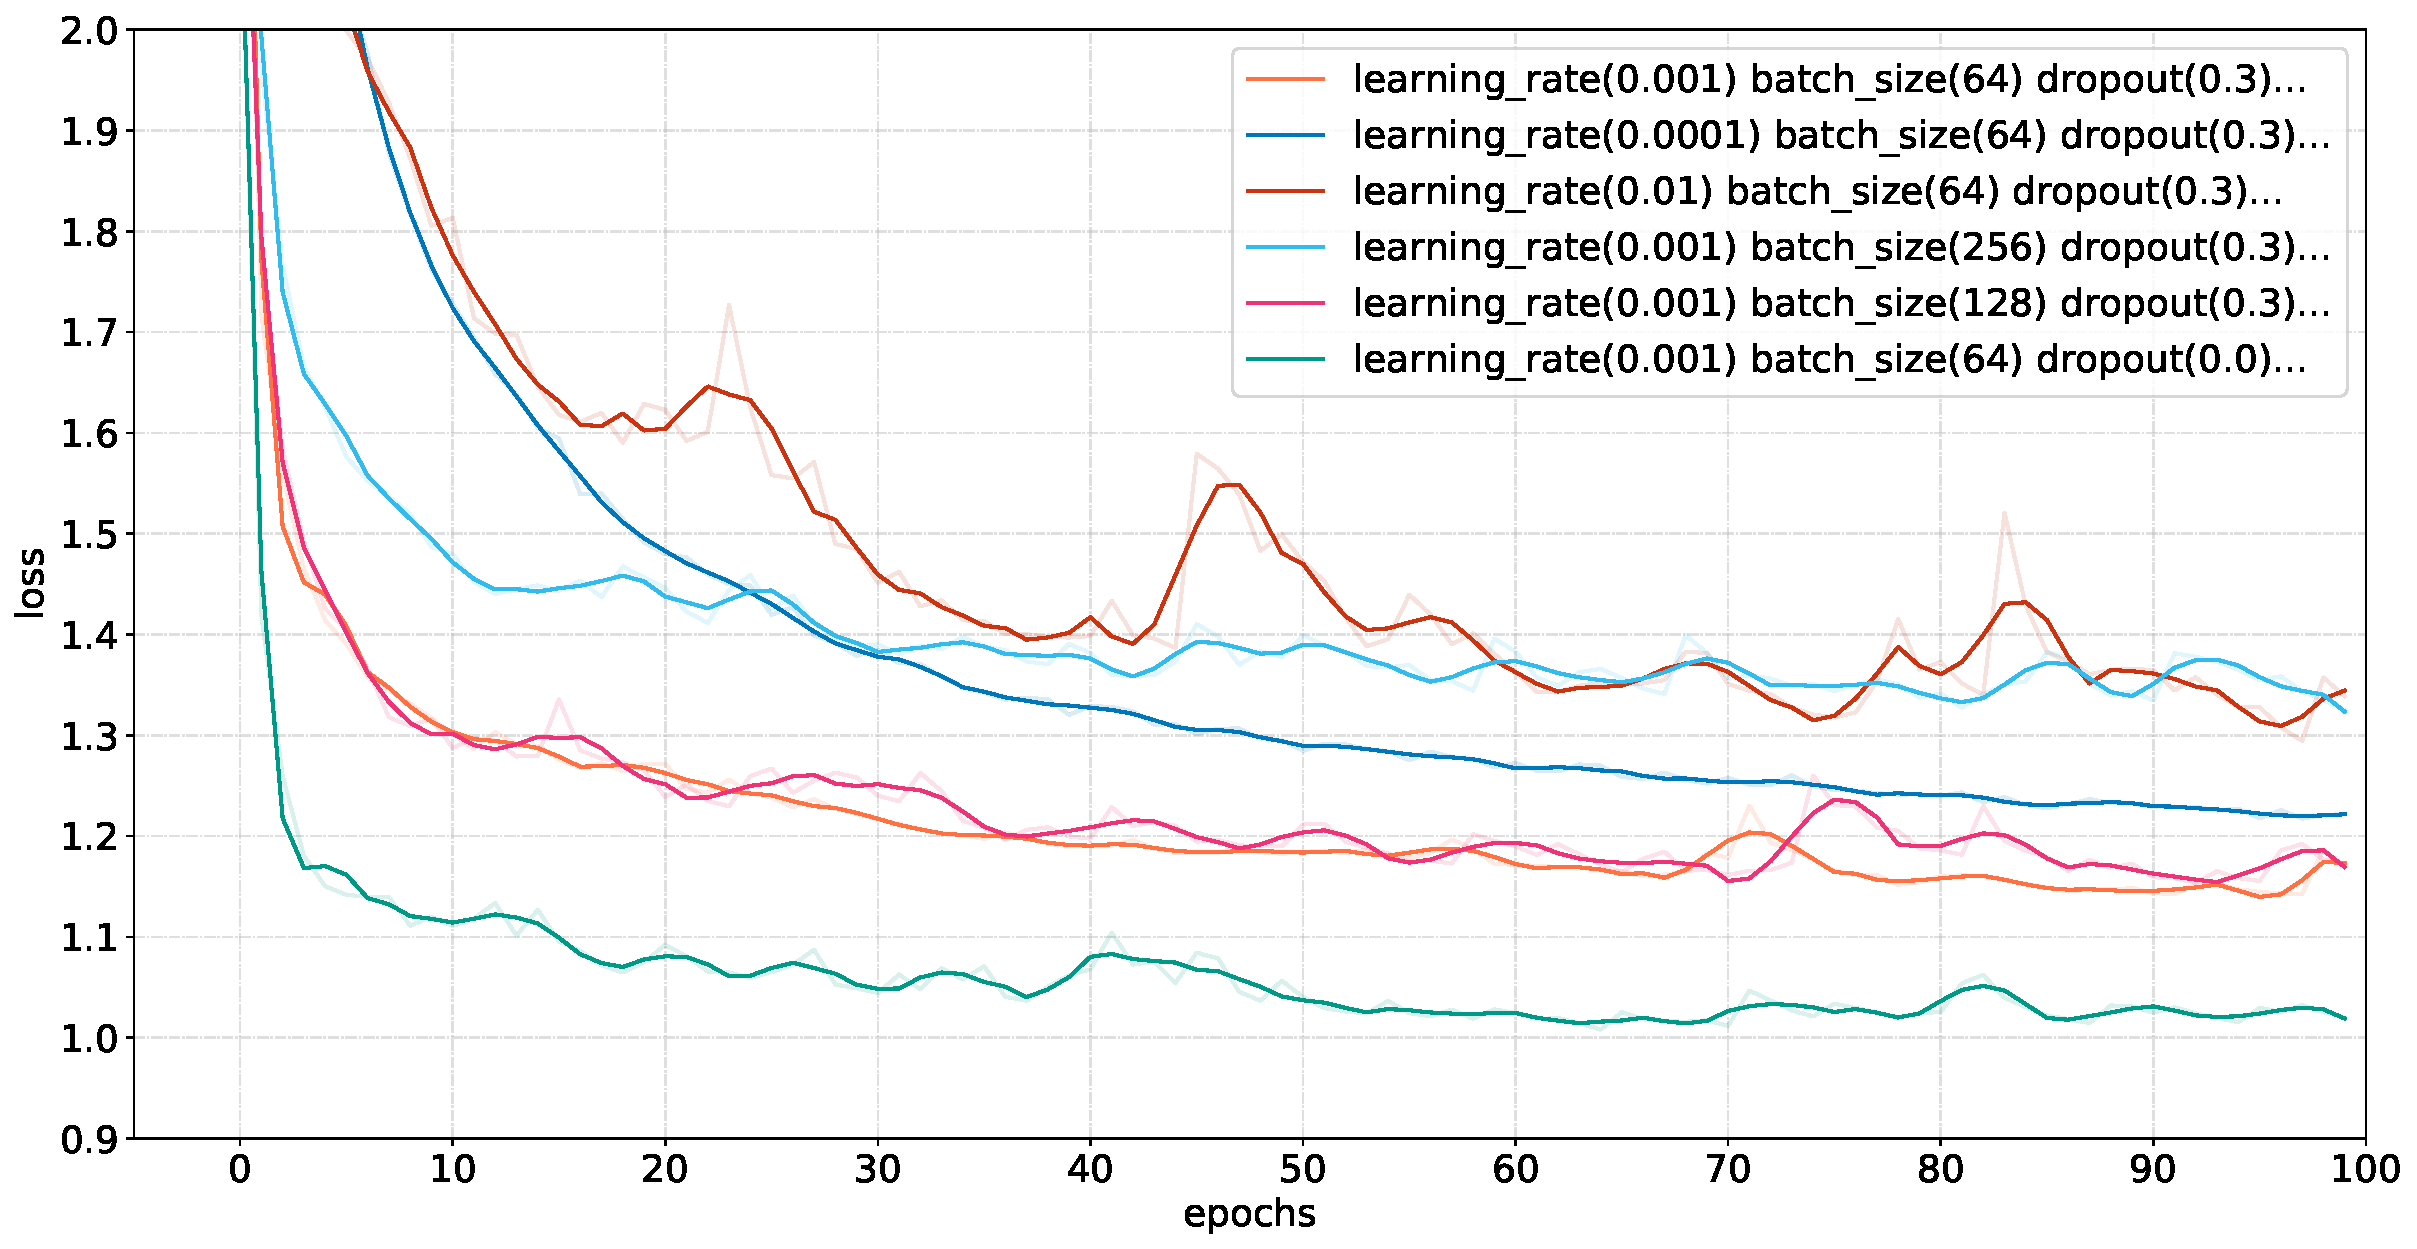
\includegraphics[width=11cm]{img/LOSS.pdf}
      \caption*{\songti 不同超参数配置下的 LOSS 变化曲线}
    \end{figure}
\end{frame}

\begin{frame}
  \frametitle{Experiments and Analysis}
    \begin{figure}
      \centering
      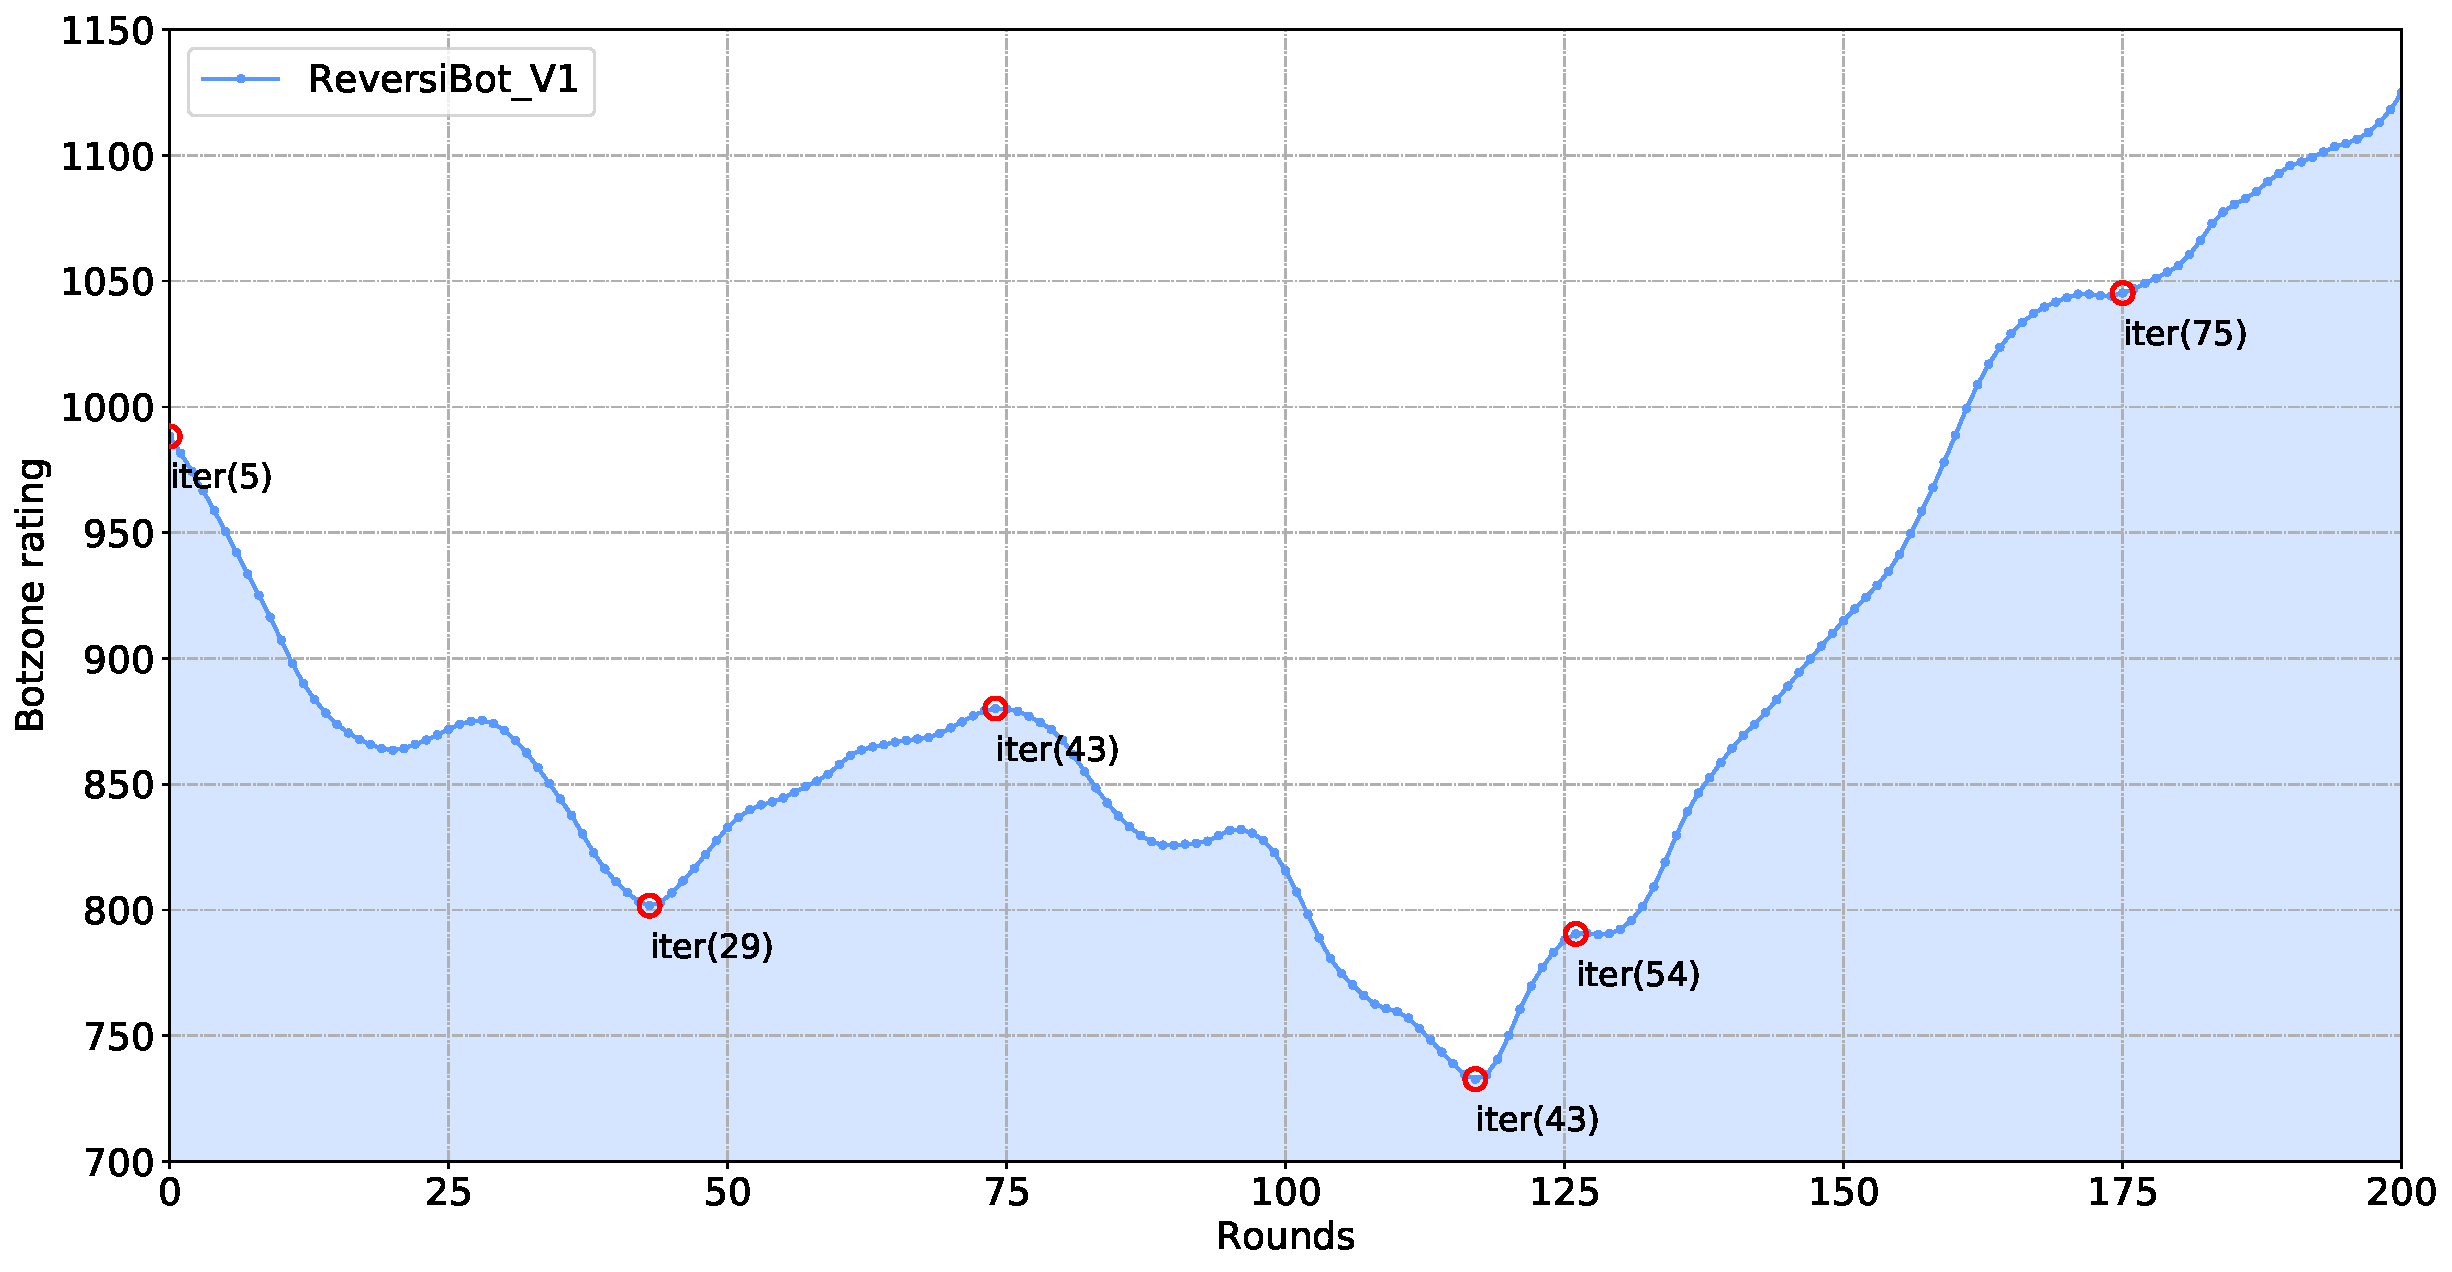
\includegraphics[width=12cm]{img/Figure_1.pdf}
      \caption*{\songti Elo rating 随迭代版本的变化曲线}
    \end{figure}
\end{frame}

\begin{frame}
  \frametitle{Experiments and Analysis}
  \begin{spacing}{1.5}
    \begin{table}[]
        \caption*{\heiti \large 不同算法实现的 AI 与本方对局结果}
        \begin{tabular}{@{}lll@{}}
        \toprule
            \multicolumn{1}{c}{\songti 基准} & \multicolumn{1}{c}{\songti 本方胜场数 / 总场数} & \multicolumn{1}{c}{\songti 本方胜率} \\ \midrule
            \songti 基于随机策略                 & 80/80                           & 100\%                    \\
            \songti 基于可转换棋子最大的贪心           & 80/80                           & 100\%                    \\
            \songti 基于使对方行动力最小的贪心          & 80/80                           & 100\%                    \\
            \songti 极大极小搜索 + Alpha-Beta 剪枝 & 56/80                           & 70\%                     \\ \bottomrule
        \end{tabular}
    \end{table}
  \end{spacing}
\end{frame}


\section{总结展望}
\begin{frame}
  \frametitle{Conclusions and Prospect}
  \textbf{一些结论}
  \begin{small}
    \begin{itemize}
      \item {\songti 人们往往认为机器学习只能在大数据的作用下发挥作用,但这是不准确的}
      \item {\songti 有些时候设计一个好的自学习算法比数据的输入更重要}
      \item {\songti 不需要任何人类知识的输入,它总是和一个与自己棋力相当的AI中对局总结经验并改进自己}
      \item {\songti 使用强化学习方法相比于传统算法预测时间短(但需预先进行训练),可提升空间大}
    \end{itemize}

    \medskip
    \textbf{期间遇到的问题(已解决)}
    \begin{itemize}
      \item {\songti Keras 多线程预测线程安全问题\textcolor{red}{(预先将图处理为静态的)}}
      \item {\songti self-play 多进程 fork 时内存资源消耗严重\textcolor{red}{(减少不必要的变量复制)}}
    \end{itemize}
    \medskip
    \textbf{展望未来}
    \begin{itemize}
      \item {\songti Dota2(多主体、不完全信息、无限状态空间),围棋(双主体、信息完全、有限状态空间)\\  % test
            即使后来的 AlphaZero 可以挑战 Dota2等相对于围棋更为复杂的游戏\\
            但它们相对于现实世界来说仍然属于简单问题}
      \item {\songti 步入强人工智能领域还需要走很长的路,也希望我们未来的生活会因此变得更加美好}
    \end{itemize}
  \end{small}
\end{frame}

\section{致谢}
\begin{frame}{Acknowledgement}
  \begin{spacing}{1.5}
    \begin{itemize}
      \item {\heiti 感谢王建华老师在毕设期间的指导}
      \item {\heiti 感谢 ACM 实验室 卢云宏老师、周世平老师、封玮老师}
      \item {\heiti 感谢班主任毕远伟老师}
      \item {\heiti 感谢四年里遇到的各位老师和同学}
    \end{itemize}
  \end{spacing}
  \medskip
  \begin{center}
    \LARGE \textbf{请多提宝贵意见}
  \end{center}
\end{frame}


\end{document}
